\documentclass[3p,review]{elsarticle}

\usepackage{lineno,hyperref}
%\usepackage{amsmath}
%\usepackage{arydshln}
\usepackage{subcaption}
%\usepackage{subfigure}
\usepackage{comment,color}
\usepackage{amssymb}

\usepackage{graphicx,amsfonts,url,multirow}
%\usepackage[cmex10]{amsmath}
\modulolinenumbers[5]

\journal{Information Fusion}

\newcommand{\TODO}{\textbf{TODO}}

%%%%%%%%%%%%%%%%%%%%%%%%%%%%%%%%%%%%%%%%%%%%%%%%%%%%%%%%%%%%%%%%%%%%%%%%%%%%%%%%%%%%%%%%%

\begin{document}

\begin{frontmatter}

\title{Big Data Analytics: A Tutorial on Information Process Fusion with MapReduce}

\author[grx]{Sergio Ram\'irez-Gallego\corref{cor1}}
\ead{sramirez@decsai.ugr.es}

\author[grx]{Alberto Fern\'andez}
\ead{alberto@decsai.ugr.es}

\author[grx]{Salvador Garc\'ia}
\ead{salvagl@decsai.ugr.es}

\author[grx]{Francisco Herrera}
\ead{herrera@decsai.ugr.es}

\address[grx]{Department of Computer Science and Artificial Intelligence, University of Granada, Granada, Spain}
%\address[kau]{Faculty of Computing and Information Technology - North Jeddah, King Abdulaziz University (KAU), Jeddah, Saudi Arabia}


\cortext[cor1]{Corresponding author. Tel:+34-958-240598; Fax: +34-958-243317}

\begin{abstract}

\TODO

%In this paper we aim at presenting the first outcomes in this framework, and to analyze the behavior of standard solutions to address imbalanced classification in Big Data problems. The features of these recent approaches, and the experimental results obtained throughout this work, will allow us to determine the current state of this area of research and to provide a discussion on the future directions. 

\end{abstract}

\begin{keyword}
Big Data Analytics, MapReduce, Information Fusion, Spark, Machine Learning
\end{keyword}

\end{frontmatter}

\section{Introduction}\label{sec:intro}

\TODO

In order to address all these objectives, this paper is organized as follows. First, Section \ref{sec:mr} presents an introduction on the MapReduce programming framework, also stressing some alternatives for Big Data processing. Section \ref{sec:techno} includes an overview on those technologies currently available to address Big Data problems from a distributed perspective. Section \ref{sec:fusion} presents the core of this paper, analyzing the different design options for developing Big Data analytics algorithms regarding how the partial data and models are aggregated. Then, we show a case study in Section \ref{sec:exp} to contrast the capabilities regarding scalability of the different approaches previously introduced. Finally, Section \ref{sec:conclusions} summarizes and concludes this paper.

\section{MapReduce as Information Process Fusion}\label{sec:mr}

The rapid growth and influx of data from private and public sectors has popularized the notion of ``Big data \cite{Fer14}''. The surge in Big Data has led to the development of custom paradigms for distributed processing that are able to extract significant value and insight in different areas such as medical, health care, business, management and so on~\cite{Kam14,Chen14,wu14}. 

Although focused on standard processing, distributed paradigms have also been widely utilized for fusing information~\cite{zhang14b, meng15} (ontologies and genetic data) and learning models~\cite{rio14b, rio15b} (trees and fuzzy rules). This section describes in detail these paradigms, putting more attention to the most widespread paradigm in the market: MapReduce. Furthermore, several examples on how MapReduce is applied as a fusion process are given here.

\subsection{MapReduce and Other Processing Paradigms}\label{subsec:mr}

%In order to provide robust and scalable solutions, new research paradigms and developmental tools have been made available. These frameworks have been designed to ease both the storage necessities and the processing of Big Data problems \cite{Fer14}. 

The MapReduce (MR) execution environment \cite{Dea08} is the most common paradigm used in the distributed processing scenario. Being a privative tool, its open source counterpart, known as Hadoop, has been traditionally used in academia research \cite{Whi15-Hadoop}. It has been designed to allow distributed computations in a transparent way for the programmer, also providing fault tolerance, automatic data partition and management, and automatic job/resource scheduling. To take advantage of this scheme, any algorithm must be divided into two main stages: Map and Reduce. The first one is devoted to split the data for processing, whereas the second collects and aggregates the results.

Additionally, the MR model is defined with respect to an essential data structure: the (key,value) pair. The processed data, the intermediate and final results work in terms of (key,value) pairs. To summarize its procedure, Figure \ref{fig:mapreduce} illustrates a typical MapReduce program with its \textit{Map} and \textit{Reduce} steps. %

%\begin{comment}
\begin{figure}[!ht]
\centering \resizebox{0.5\textwidth}{!}{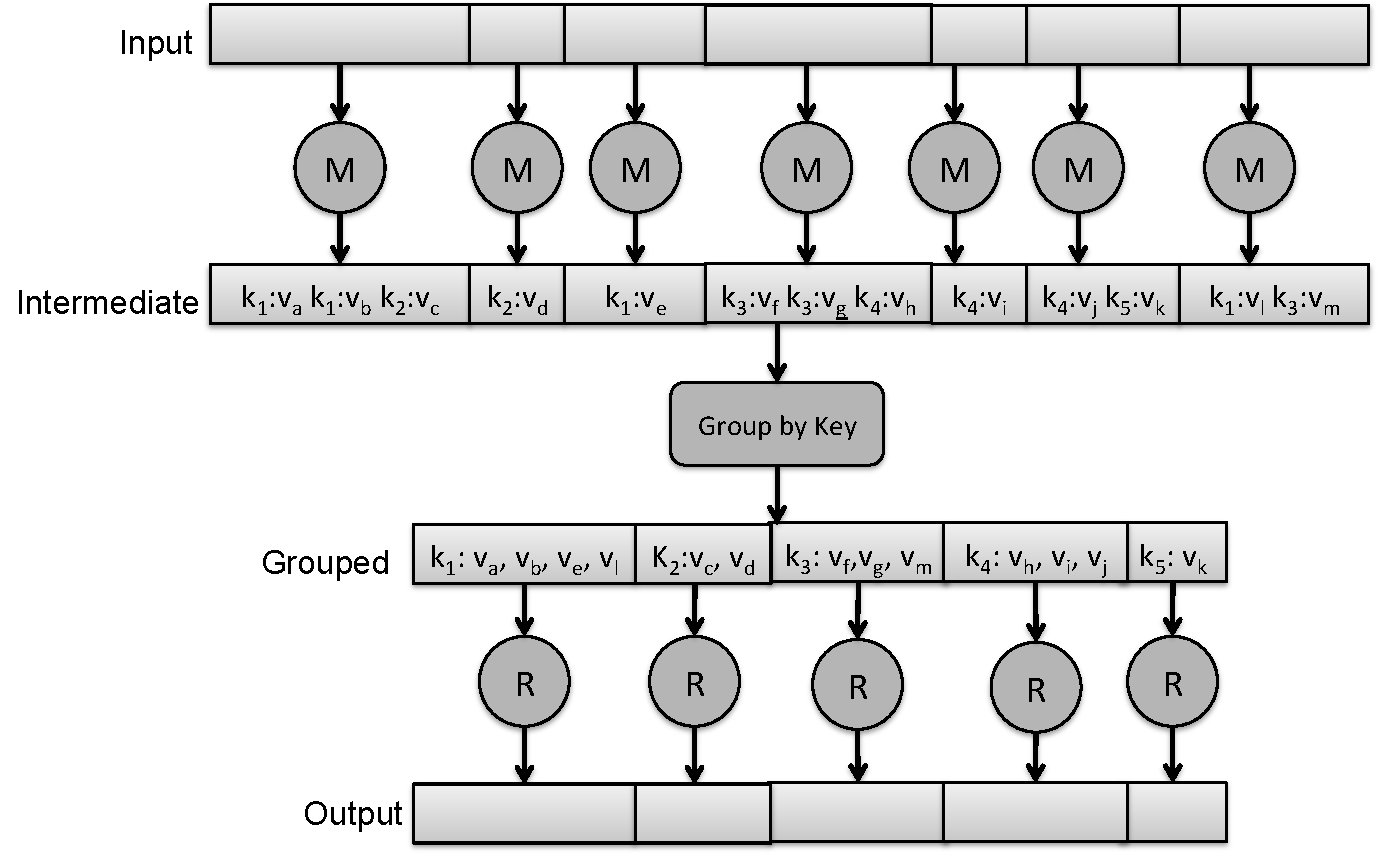
\includegraphics{mapreduce}} \caption{The MapReduce programming model. $k$ elements represent the keys in the pairs, whereas $v$ the values.}
\label{fig:mapreduce}
\end{figure}
%\end{comment}

The MR scheme can be described as follows. Map function first reads data and transforms records into a key-value format. Transformations in this phase may apply any sequence of operations on each record before sending the tuples across the network. Output keys are then shuffled and grouped by key value so that coincident keys are grouped together to form a list of values. Keys are then partitioned and sent to the Reducers according to some key-based scheme previously defined. Finally, the Reducers perform some kind of aggregation on the lists to eventually generate a single value for each pair. As a further optimization, the reducer is also used as a combiner on the map outputs. This improvement reduces the total amount of data sent across the network by combining each word generated in the Map phase into a single pair.

%The terms $k_i:v_j$ refer to the key and value pair that are computed within each Map process. Then, values are grouped linking them to the same key, i.e. $k_i:v_j,\ldots, v_h$, and feed to the same Reduce process. Finally, values are aggregated with any function within the Reduce process to obtain the final result of the algorithm.

Apart from considering MR as a processing paradigm, this scheme (concretely, the Reduce stage) can also be seen as a fusion process that allows to blend partial models and information schemes into a final fused outcome. Fusion of models in MR is typically performed following some sort of ensemble strategy that combine multiple hypothesis through voting or attachment. Also exist other proposals that go beyond ensemble learning, and offers as outcome a single coalesced model. For example, logistic regression in Spark is composed by several subgradients that are locally computed and eventually aggregated (more examples in Section~\ref{sec:fusion}). In case of information, fusion process is more dependent from the input domain and the diversity of cases is highly diverse. Use cases for MR in the literature range from fusion of ontologies~\cite{zhang14b} to the composition of fuzzy rules~\cite{rio15b}.

Word Count comes to be one of the most widespread examples to illustrate the intrinsic information fusion process behind MR. WordCount is intended to count the number of occurrences per word in a set of input text files. Each mapper reads a set of blocks formed by lines, and splits them into words. It then emits a key-value pair with the word as key, and 1 as value. Afterwards, each reducer sums the scores for each word, and outputs a single key-value pair with the word and sum. 

Consider the phrase "knock, knock, who is there?". A single mapper would receive and split this sentence as words, and then, it would form the initial pairs as: (knock,1), (knock,1), (who,1), (is,1), (there,1). In reducers, the keys are grouped together and the count values for identical keys (words) are added. In this case only one pair of similar keys `knock' would be aggregated so that the output pairs would be as follows: (knock,2), (who,1), (is,1), (there,1). As result, the user would receive the final number of hits for each word. 

Mahout's Random Forest is a good example of how ensemble learning is performed on Hadoop. Although very simple, it will serve us to illustrate the behavior of information fusion in MR. The algorithm consist of two MR phases: the first one is devoted to the development of the model (where model fusion occurs), and the second one is focused on class prediction once the model is built.

In the first phase, each Map creates several random trees (a subset of the forest) using the partitions given as input. The reduce phase simply concatenates all the trees forming the final forest of random trees. The second task replicates the forest across the nodes, and launches the mappers on the test set partitions. Mappers predict the class for each record assigned by using the final model. Finally, reducers concatenate predictions in a single file.

%Despite these limitations, many Big Data technologies provide a wrapper implementation of MapReduce for end users (like Spark) due to its great popularity.


\subsection{Alternatives}\label{subsec:altMR}

Although MR is the most popular paradigm to tackle distributed processing, there exist other modern distributed frameworks, conceived prior to the dawn of MR, that offer other alternatives for information and model fusion. Most of them follows a Single Instruction Multiple Datasets (SIMD)~\cite{sung00} scheme to execute the same sequence of instructions simultaneously on a distributed set of data partitions. In this section we focus on two paradigms (graph and bulk processing) relevant for current Big Data platforms.

\subsubsection{Directed Acyclic Graph Parallel Processing}

All distributed frameworks based on Directed Acyclic Graph (DAG)~\cite{dennis74}, like Spark, organize their jobs by splitting them into a smaller set of atomic tasks. In this model vertices correspond with parallel tasks, whereas edges are associated with exchange of information. As shown in Figure~\ref{fig:dag}, vertices can have multiple connections between inputs and outputs, which imply that the same task can be run in different data and the same data in different partitions. Data flows are physically supported by shared memory, pipes, or disks. Instructions are duplicated and sent from the master to the slave nodes for a parallel execution. Notice that MR can be deemed as an specific implementation of DAG-based processing, with only two functions as vertices. 

\begin{figure*}[htp]
    \centering
    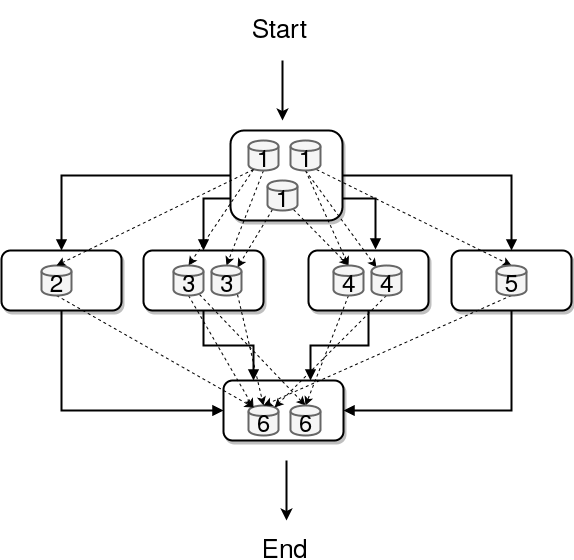
\includegraphics[width=0.4\textwidth]{dag}
    \caption{Direct Acyclic Graph Parallel Processing. Squares represent the tasks to process and the nodes in the graph, arrows connecting nodes represent the data flow between nodes and the vertices in the graph, dashed lines represent the dependencies between data blocks (cylinders).}
    \label{fig:dag}
\end{figure*}

%Figure~\ref{fig:dag} depicts a DAG execution program with 4 tasks, and different partition configuration for each task. For instance, the top-most task in the graph is formed by 3 partitions. Once this task has finished, two dependent tasks (3 and 4) are started. Dependencies between partitions are not trivial as can be seen in the figure. Right-most partition in task 2 only depends on two input partitions, whereas left-most partitions has a single dependency. Finally, the input of task 4 is connected with the output of task 2 and 3. It is thus noteworthy to remark the differences between data (black dashed lines) and task dependencies (blue lines).

\subsubsection{Bulk Synchronous Parallel Processing}

Bulk Synchronous Parallel (BSP)~\cite{vali90} systems are formed by a series of connected supersteps, implemented as directed graphs. In this scheme input data is the starting point. From here to the end, a set of Supersteps are applied on partitioned data in order to obtain the final output. As mentioned before, each Superstep correspond with an independent graph associated with a subtask to be solved. Once all compounding subtasks end, bulk synchronization of all outputs is committed. At this point vertices may send messages to the next Superstep, or receive some from previous steps, and also to modify its state and outgoing edges. Figure~\ref{fig:bsp} shows a toy example for BSP processing with two Supersteps and one synchronization barrier.

\begin{figure*}[htp]
    \centering
    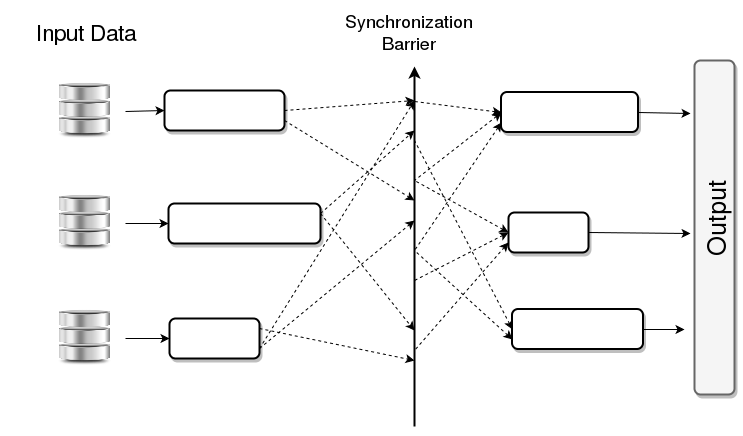
\includegraphics[width=0.5\textwidth]{bsp}
    \caption{Bulk Synchronous Parallel Processing. Subtasks in each Superstep are depicted as rectangles with variable height (task duration), and data flows as dashed lines. Synchronization barrier acts as a time proxy between stages.}
    \label{fig:bsp}
\end{figure*}

\section{Big Data Technologies for Analytics}\label{sec:techno}


Nowadays, the volume of data currently managed by our storage systems have surpassed the processing capacity of traditional systems~\cite{wu14}, and this applies to data mining as well. Distributed computing has been widely used by data scientists before the advent of Big Data to boost up sequential solutions in medium-size data. Nevertheless, for most of current massive problems, a distributed approach becomes mandatory nowadays since no batch architecture is able to address such magnitudes.

Beyond High Performance Computing (HPC) solutions, new large-scale processing platforms are intended to bring closer distributed processing to practitioners and experts by hiding the technical nuances derived from these environments. Novel and complex designs are required to create and maintain these platforms, which generalizes the utilization of distributed computing for standard users. 

As a result of the fast evolving of Big Data environment, a myriad of tools, paradigms and techniques have surged to tackle different use cases in industry and science. However, because of the myriad of tools, it is often difficult for practitioners and experts to analyze and select the right tool for each goal. In this section we present and analyze some alternatives for distributed processing with the objective of providing the necessary knowledge that helps users to decide which alternative better fits their requirements. We also outline the software libraries that gives support to the distributed learning task in these platforms.

\subsection{Apache Hadoop}\label{subsec:hadoop}

Undoubtedly Hadoop MapReduce may be deemed as the primary platform in the Big Data space. After the presentation of MR by Google designers~\cite{dean04}, Hadoop MapReduce was grown by the community, and became the most used and powerful open-source implementation of MR. Nowadays leading companies such as Yahoo has scaled from 100-node Hadoop clusters to 42K nodes and hundreds of petabytes~\cite{harris13} thanks to the outstanding performance of Hadoop. 

The main idea behind Hadoop was to create a common framework which can process large-scale data on a cluster of commodity hardware, without incurring in a high cost in developing (in contrast to HPC solutions) and execution time. Hadoop MapReduce was originally composed by two elements: the first one was a distributed storage system called Hadoop Distributed File System (HDFS), whereas the second one was a data processing framework that allows to run MR-like jobs. Apart from these goals, Hadoop implements primitives to address cluster scalability, failure recovery, and resource scheduling, among others.

But Hadoop is today more than a single technology, but a complete software stack and ecosystem formed by several top-level components that address diverse purposes. For instance, Apache Giraph for graph processing or Apache Hive for data warehousing. The common factor is that all of them rely on Hadoop, and are tightly linked to this technology. Some projects are actually Apache top-level projects~\cite{apache}, whereas others are continuously evolving or being created.%In this section, we focus on enumerating the main components of Hadoop, as well as the cutting-edge elements recently developed for the ecosystem. %All components are divided into several categories: storage, processing, high-level components. Figure~\ref{fig:hadoopeco} depicts a simplified scheme with the most popular components.

\textbf{HDFS}~\cite{hdfs} can be deemed as the main module of Apache Hadoop. It supports distributed storage for large-scale data through the use of distributed files, which themselves are composed by fixed-size data blocks. These blocks or partitions are equally distributed among the data nodes in order to balance as much as possible the overall disk usage in the cluster. HDFS also allows replication of blocks across different nodes and racks. In HDFS, the first block is ensured to be placed in the same processing node, whereas the other two replicas are sent to different racks to prevent abrupt ends due to inter-rack issues. 

HDFS was thought to work with several storage formats. It offers several APIs to read/write registers. Some relevant APIs are: InputFormat (to read customizable registers), or RecordWriter (to write record-shaped elements). Users can also developed their own storage format, and to compress data according to their requirements. Persistence in Hadoop is mainly performed in disk. However, there are some novel advances to optimize persistence by introducing some memory usage. For instance, in Apache Hadoop version 3.0 was introduced the option of memory usage as temporary storage.

Although~\textbf{MR}~\cite{dean04} is the native processing solution in Apache Hadoop, today it supports multiple alternatives with different processing schemes. All these solutions have in common that use a set of data nodes to run tasks on the local data blocks, and one master node (or more) to coordinate these tasks. For instance,~\textbf{Apache Tez}~\cite{tez} is a processing engine that transforms processing jobs into direct acyclic graphs (DAGs). Thanks to Tez, users can run any arbitrary complex DAG of jobs in HDFS. Tez thus efficiently solves interactive and iterative processes, like those present in machine learning processes. Its most relevant contribution is that Tez translate any complex job to a single MR phase. Furthermore, it does not need to store intermediate files and reuses idle resources, which highly boost the overall performance.

Hadoop MapReduce evolves to a more general component, called \textbf{Yet Another Resource Negotiator (YARN)}~\cite{yarn}, which provides extra management and maintenance services relied to other components in the past. YARN also acts as a facade for different types of distributed processing engines based on HDFS, such as Spark, Flink or Storm. In short, YARN was intended as a generic purpose system that separates the responsibilities of resource management (performed by YARN), and running management (performed by top-level applications).

Among the full set of advantages claimed by YARN, we can highlight its capacity to run several application on the same cluster without the necessity of moving data. In fact, YARN allows reusing resources across alike applications in parallel, which improves the overall usage of resources.

\subsubsection{Apache Mahout}

Since the magnitude of learning problems has been growing exponentially, data scientists demands rapid tools that efficiently extract knowledge from large-scale data. This problem has been solved by MR and other platforms by providing scalable algorithms and miscellaneous utilities in form of machine learning libraries. These libraries are compatible with the main Hadoop engine, and use as input the data stored in the storage components. 

\textbf{Apache Mahout}~\cite{mahout} was the main contribution from Apache Hadoop to this field. Although it can be deemed as mainly obsolete nowadays, Mahout is considered as the first attempt to fill the gap of scalable machine learning support for Big Data. Mahout comprises several algorithms for plenty of tasks, such as: classification, clustering, pattern-mining, etc. Among a long list of golden algorithms in Mahout, we can highlight Random Forest or Na\"ive Bayes. 

The most recent version (0.13.0) provides three new major features: novel support for Apache Spark and Flink, a vector math experimentation for R, and GPU support based on large matrix multiplications. Although Mahout was originally designed for Hadoop, some algorithms have been implemented on Spark as a consequence of the latter one's popularity. Mahout is also able to run on top of Flink, being only compatible for static processing though.

\subsection{Spark}\label{subsec:spark}

\textbf{Apache Spark Framework}~\cite{spark} was born in 2010 with the publication of Resilient Distributed Datasets (RDD) structures~\cite{zaharia12}, the keystone behind Spark. Although Spark has a close relationship with Hadoop Ecosystem, it provides specific support for every step in the Big Data stack, such as its own processing engine, and machine learning library. 

Apache Spark~\cite{hamstra15} is defined as a distributed computing platform which can process large volume data sets in memory with a very fast response time due to its memory-intensive scheme. It was originally thought to tackle problems deemed as unsuitable for previous disk-based engines like Hadoop. Continued use of disk is replaced in Spark by memory-based operators that efficiently deal with iterative and interactive problems (prone to multiple I/O operations). 

%RDD
The heart of Spark is formed by \textbf{Resilient Distributed Datasets (RDD)}, which transparently controls how data are distributed and transformed across the cluster. Users just need to define some high-level functions that will be applied and managed by RDDs. These elements are created whenever data are read from any source, or as a result of a transformation. RDDs consist of a collection of data partitions distributed across several data nodes. A wide range of operations are provided for transforming RDDs, such as: filtering, grouping, set operations, among others. Furthermore RDDs are also highly versatile as they allows users to customize partitioning for an optimized data placement, or to preserve data in several formats and contexts.

% lineage
In Spark, fault tolerance is solved by annotating operations in a structure called lineage. Spark transformations annotated in the lineage are only performed whenever a trigger I/O operations appears in the log. In case of failure, Spark re-computes the affected brach in the lineage log. Although replication is normally skipped, Spark allows to spill data in local disk in case the memory capacity is not sufficient. 

%Dataframes
Spark developers provided another high-level abstraction, called \textbf{DataFrames}, which introduces the concept of formal schema in RDDs. DataFrames are distributed and structured collections of data organized by named columns. They can be seen as a table in a relational database or a dataframe in R, or Python (Pandas). As a plus, relational query plans built by DataFrames are optimized by the Spark's Catalyst optimizer throughout the previously defined schema. Also thanks to the scheme, Spark is able to understand data and remove costly Java serialization actions.

%Datasets
A compromise between structure awareness and the optimization benefits of Catalyst is achieved by the novel Dataset API. \textbf{Datasets} are strongly typed collections of objects connected to a relational schema. Among the benefits of Datasets, we can find compile-time type safety, which means applications can be sanitized before running. Furthermore, Datasets provide encoders for free to directly convert JVM objects to the binary tabular Tungsten format. These efficient in-memory format improves memory usage, and allows to directly apply operations on serialized data. Datasets are intended to be the single interface in future Spark for handling data.

\subsubsection{MLlib}


\textbf{MLlib} project~\cite{mllib15} was born in 2012 as an extra component of Spark. It was released and open-sourced in 2013 under the Apache 2.0 license. From its inception, the number of contributions and people involved in the project have been growing steadily. Apart from official API, Spark provides a community package index~\cite{sparkpackages} (Spark Packages) to assemble all open source algorithms that work with MLlib. 

MLlib is a Spark library geared towards offering distributed machine learning support to Spark engine. This library includes several out-of-the-box algorithms for alike tasks, such as: classification, clustering, regression, recommendation, even data preprocessing. Apart from distributed implementations of standard algorithms, MLlib offers:

\begin{itemize}
	\item Common Utilities: for distributed linear algebra, statistical analysis, internal format for model export, data generators, etc. 
	\item Algorithmic optimizations: from the long list of optimizations included, we can highlight some: decisions trees, which borrow some ideas from PLANET project~\cite{panda09} (parallelized learning both within trees and across them); or generalized linear models, which benefit from employing fast C++-based linear algebra for internal computations.
	\item Pipeline API: as the learning process in large-scale datasets is tedious and expensive, MLlib includes an internal package (\emph{spark.ml}) that provides an uniform high-level API to create complex multi-stage pipelines that connect several and alike components (preprocessing, learning, evaluation, etc.). \emph{spark.ml} allows model selection or hyper-parameter tuning, and different validations strategies like k-fold cross validation.
	\item Spark integration: MLlib is perfectly integrated with other Spark components. Spark GraphX has several graph-based implementations in MLlib, like LDA. Likewise, several algorithms for online learning are available in Spark Streaming, such as online k-Means. In any case, most of component in the Spark stack are prepared to effortlessly cooperate with MLlib.
\end{itemize}

\subsection{Flink}\label{subsec:flink}

\textbf{Apache Flink}~\cite{flink} is a distributed processing component focused on streaming processing, which was designed to solve problems derived from micro-batch models (Spark Streaming). Flink also supports batch data processing with programming abstractions in Java and Scala, though it is treated as a special case of streaming processing. In Flink, every job is implemented as a stream computation, and every task is executed as cyclic data flow with several iterations. 

Flink provides two operators for iterations~\cite{flinkengine}, namely, standard and delta iterator. In standard iterator, Flink only works with a single partial solution, whereas delta iterator utilizes two worksets: the next entry set to process and the solution set.
Among the set of advantages provided by iterators is the reduction of data to be computed and sent between nodes \cite{EwenTKM12}. According to the authors, new iterators are specially designed to tackle machine learning and data mining problems.

Apart from iterators, Flink leverages from a PACT optimizer which analyzes the code and the data access conflicts to reorder operators and create semantically equivalent execution plans~\cite{Alexandrov14,Hues12}. Physical optimization is then applied on plans to boost data transport and operators' execution on nodes. Finally, PACT optimizer selects the most resource-efficient plan, regarding network and storage.

Furthermore, Flink provides a complex fault tolerance mechanism to consistently recover the state of data streaming applications. This mechanism is generating consistent snapshots of the distributed data stream and operator state. In case of failure, the system can fall back to these snapshots.

\textbf{FlinkML} is aimed at providing a set of scalable ML algorithms and an intuitive API to Flink users. Until now, FlinkML provides few alternatives for some fields in machine learning: SVM with CoCoA~\cite{jaggi14}, or Multiple Linear regression for supervised learning, k-NN join for unsupervised learning, scalers and polynomial features for preprocessing, Alternating Least Squares for recommendation, and other utilities for validation and outlier selection, among others. FlinkML also allows users to build complex analysis pipelines via chaining operations (like in MLlib). FlinkML pipelines are inspired by the design introduced by sklearn in~\cite{buitin13}.

\section{Big Data Analytics on Fusion Process}\label{sec:fusion}

``Synchronizing flags'' in every distributed algorithmic approach is undoubtedly the most challenging part during the design process. This issue is not an exception in the MapReduce scheme. In this particular case, developers must take two significant decisions. On the one hand, the components selected for the key-value representation in both the Map and Reduce input and outputs. On the other hand, how the list of values are aggregated in the Reduce step. 

For Big Data applications in Machine Learning, these choices are of extreme importance for the behavior of the final models. In this section, we want to analyze in detail this characteristic of the MapReduce programming environment by introducing a taxonomy to organize current state-of-the-art approaches regarding how partial models from the Map task are aggregated. We will determine how this fact may also affects the actual scalability of the whole system. 

Specifically, we distinguish among three different type of models. First, those that carry out a direct fusion of partial models, thus becoming and ensemble system (Section \ref{subsec:ensemble}). Second, those that create a partial model within different Maps, and combine them to obtain a single output (Section \ref{subsec:submodels}). Finally, we identify those designs which distribute both data and sub-models to iteratively build the final system (Section \ref{subsec:exact}).

\subsection{Direct fusion of models: ensemble approach}\label{subsec:ensemble}

In every MapReduce framework, the system partitions the input training data to feed the Map functions. This computational paradigm reminds of the traditional \textit{bootstrap aggregating} (bagging) approach; in this case with no replacement. Therefore, it is straightforward to obtain an ensemble-based classifier \cite{Polikar2006} by directly joining every single model obtained in a different Map task. 

The premise for this type of methodologies is simple yet effective. Each Map task works independently on its chunk of data. Depending on the user's requirements, each Map function is devoted to build a one or more models. For example, a pool of 100 classifiers to be obtained from 5 Maps will result on 20 classifiers per Map, each one of them built from a 20\% of the original dataset. The ``key'' is shared by all values given as output from the Map. This fact makes the logic of the Reduce phase to stress for its simplicity. Every single classifier is directly joined into the final system. 

There are two main advantages for this type of design. On the one hand, we have stressed its direct synergy with the MapReduce programming model, easing the programmer implementation. On the other hand, we must refer to the degree of diversity of those models obtained from different Maps, being a crucial characteristic for the success of these types of methods \cite{Kuncheva05}. 

In spite of the previous goodness, there is one significant problem: there is a limit in the scalability degree. It must be acknowledge that there is a strong relationship between the number of Maps and the required number of models. In other words, we cannot decrease the total running time by adding a larger number of Maps, as this may result in ``void'' functions with a data input but no output. 

One final drawback that must be stressed is related to the inner concept of ensemble. Being composed of a ``large'' set of individual models, two facts must be taken into account. On the one hand, since all of them are considered for the classification step, it is hard to understand the actual reason for the labeling of the queried data. On the other hand, the robustness of the whole ensemble system somehow depends on the individual quality of its components, as well as their diversity. Both properties are not easy to hold, and impose a restriction in the building of the ensemble, for both standard and Big Data applications.

\subsection{Approximate fusion of models: aggregation of partial systems}\label{subsec:submodels}

As it was pointed out in the previous section, one straightforward way to design an scalable algorithm is trying to compute independent parallel tasks, i.e. to avoid data exchange between nodes. By carrying out separate computations within each Map task, complete models are obtained, all of which could work directly over the test data, as they maintain no a priori relationship among them. %Finally, the computational cost of each chunk could be so high that a fault-tolerant mechanism is mandatory. 

To empower the recognition ability of these single models, their combination into an ensemble system has been suggested. However, we have also emphasized several some problems related to this design. In order to address or at least alleviate them, one possible solution is trying to aggregate these partial systems into a single model. 

The hitch in this case is how to design the Reduce function in order to combine the individual models coming from each Map. In order to have an insight on the possible alternatives to overcome this problem, some significant proposals given in the specialized literature will be described next.

%%Corregidme si me equivoco
A first example is the clustering procedure by means of a standard k-Means \cite{Zhao09-kMeans}. Each Map process is devoted to compute the nearest samples (from its input chunk of data) to each of the $k$ centroids (initially set at random). The output key-value is the centroid ``id'' and the attributes of the nearest sample respectively. Then, each Reducer recalculates the new centroids coordinates by averaging the values of those samples given as ``list of values'' for each key (centroid). The whole procedure is then iterated in order to refine the centroids, thus improving their robustness. It must be observed the importance of the Reduce step for the global combination of the partial information computed within each Map.  

k-Nearest Neighbor (kNN) classifier \cite{MailloRTH17-kNN} has also some points in common with clustering, as it is based on distances among examples. In this case, the Map stage is devoted to obtain the $k$ nearest training instances to each query input. To carry out an exact computation, the whole test set should be given as input to each Map, allowing to obtain as key-value the index of the test instance and a list of the $k$ closest distances with their corresponding training class labels. Then, the Reducer only needs to find, among all $M$ sets of $k$-nearest neighbors (with $M$ the number of Maps) the one with lowest value to finally assign the output class.

Prototype Reduction \cite{TrigueroPBGH15-PR} is also a significant example in this context. First, each Map process works with a different chunk of data by applying any available reduction procedure \cite{TrigueroDGH12}. Then, selected prototypes are fed to a single reducer that is devoted to eliminate redundant ones. This implies a clear fusion of data in order to obtain a final model, in this case merging similar examples. 

The information-based feature selection framework (IFSF) proposed in~\cite{Ramirez-Gallego17-mrmr} is an example of how submodels (importance by feature) can be fused in data preprocessing. This multivariate algorithm measures redundancy and relevance between the input features and the output class in order to elect a reduced set of relevant features. As a first step in IFSF, input data is vertically split to strictly separate computations between features. Then, feature interactions are modeled by replicating the last selected feature and the class across the nodes so that the minimum amount of communication is performed. The map stage calculates the feature scores individually, and the reduce stage selects the best feature from the current set of unselected features.


Another interesting approaches come from the boosting perspective \cite{schapire99brief}, which are AdaBoost.PL, LogitBoost.PL and MultiBoost.PL \cite{Palit12-Boost}. These include an ensemble of ternary classifiers \cite{schapire99confidence}, or an ensemble of ensembles. Although it can be wrongly associated with those methods introduced in the previous section, these have been included in this type of methodology regarding the functionality implemented within the Reduce step. Specifically, the whole boosting procedure, i.e. $T$ iterations, is carried out within each Map, so $M$ ensemble of $T$ classifiers are obtained, being $M$ the number of maps. Then, the $T$ classifiers are arranged according to their score, i.e. the weighted error, and then emitted to the Reducers using their index as ``key'' and the model as value. Finally, each Reduce process takes all classifiers with the same index (key) and compute an average weight for this ensemble. At classification time, each ``sub-ensemble'' provides a vote for its class, whose value is exactly the aforementioned weighted average score.  

Fuzzy Rule Based Classification Systems \cite{Fer16_fuzzyBD} are probably one of the clearest type of models in this category. The pioneer implementation was based on the Chi et al approach \cite{RioLBH15-Fuzzy}. Each Map task comprises a complete fuzzy learning procedure to obtain an independent Rule Base (RB). To do so, all examples from the input data chunk are iterated deriving a single rule per example, while merging those with the same antecedent and consequent. Then, rule weights (RWs) are computed based on a fuzzy confidence value from the input examples, also allowing to determine the output class. We must acknowledge that at this stage every single RB might be used for classification purposes. However, the system can be further enhanced by combining all partial models for every Map, as stated in the beginning of this section. To do so, the Map writes as key-value pair the antecedent and consequent (including class and RW) respectively. Reducers then merges those rules with the same antecedent (key) by averaging the values of the RWs for the same class consequents, and then the class with the highest RW is finally maintained. 

%\cite{SongRHM15}

Throughout this section we have presented a short overview on those MapReduce methods that are based on fusion of partial models. As such, they allow to reinforce the abilities of those individual systems, leading to possibly more robust approaches. However, two issues must be taken into account:

\begin{enumerate}
\item The key-value representation to link the Map and Reduce processes. It must be very carefully selected as it has a strong influence in the design of the Map function. Although the procedure is usually implemented to be independent among Maps, a common point should be given in order to allow the final combination. 

\item The aggregation function in the Reducer. It has a clear dependence on the previous item, so that these must be designed as a whole to ensure a robust workflow.

\end{enumerate}

Both points will determine the scalability and exactness of the output system. We refer to the changes in behavior when increasing the number of Maps. Specifically, the efforts must be mostly focused on the development of the partial models, regarding the influence of the lack of data and/or whether the knowledge acquired from different subsets of the problem space are able to be accurately merged.

\subsection{Exact fusion for scalable models: distributed data and models' partition}\label{subsec:exact}

The previous scheme based on fusion of submodels is presented as ideal for distributed learning since submodel creation is naturally parallelizable, and the subsequent final model can be deemed as exact. Nevertheless, this kind of fusion is rarely applied since creation and/or fusion of partial models is only feasible in a scarce set of problems. For instance, most of supervised methods demand to access to a large percentage of instances (usually, the whole set) during the training step. In this case, submodel creation is not possible because of the strong dependency between data partitions. 

Decision trees (DT), as supervised algorithms, are not originally designed to support partial construction in the distributed environment. They are top-down algorithms that continuously evaluate splits by using statistics sketches computed on the entire dataset. In this case, all instances (and data partitions) are involved on the statistics computation at every step, except in the rare scenario where all feature values in a partition belongs to leaves nodes. Parallelization here is then considered as a more complex task.

A possible solution to this problem is to utilize partitioned data to make decisions about how to construct a single exact model. For DTs, statistics for each split considered are collected from the datanodes, and used in the master node to decide which split is the best option for the current state of the model.

This scheme was originally implemented in the Parallel Learner for Assembling Numerous
Ensemble Trees (PLANET) method~\cite{Panda09-DT-RF}. In \textbf{PLANET}, master node controls the complete tree induction process, and launches the MR jobs that construct the nodes. It also maintains the tree model in memory, decides which split predicates will be evaluated, and eventually replicates the updated model across the nodes. Nodes to be evaluated are organized through several queues, one with nodes for MR-based evaluation and another for in-memory evaluation. Depending on the amount of instances involved in computations, nodes are pushed to one queue or the other. Here we focus on MR evaluation of nodes which is more common.

As tree construction proceeds, the master node retrieves nodes from the queue, and schedules MR jobs to evaluate splits. Inside these jobs, statistics for splits are computed in the map side by using the instances in the data partitions. Finally, the reduce side decides which split is more convenient for the tree model. Once a MR job ends, the master nodes updates the model with the nodes and the splits predicates selected, and updates the queues with new nodes at the periphery.

Notice that in this scheme, each MR job fetches the entire dataset in order to avoid determining which records are required by each node, and the extra communication that this step conveys. Instead, it performs a level-wise computation of splits so that the tree is constructed by following a breadth-first strategy. Thanks to this scheme, all nodes at a given level are expanded at the same step, and every instance is part of the input to some analyzed node.

PLANET project does not only offer an elegant solution for single tree induction, but it also extends the original idea to provide powerful exact algorithms based on \textbf{bagging} and \textbf{boosting} ensembles~\cite{hastie11}. Concerning bagging, PLANET allows to build multiple trees by maintaining a single queue of nodes for the whole set of trees. By alternating evaluation of nodes from several trees, PLANET can build the random forest in a parallel way. During boosting, PLANET constructs weak learners sequentially as usual. Here training is only parallelized at the tree level. Residuals are easily computed since the model is sent to every MR job in full.

Based on PLANET, MLlib' creators~\cite{mllib15} developed two ensemble classifiers for exact fusion: one based on random forest of trees, and another based on gradient boosted trees~\cite{mllibtrees}. Standard DTs are also adopted in MLlib, however, note that they are implemented as an singular case of random forest with a single tree and the full feature set. In general, all aforementioned tree-based algorithms have incorporated several optimizations~\cite{mllibdt} with respect to PLANET, intended to boost up the tree induction process. Major features introduced are describe below:

\begin{itemize}
	\item \textit{Efficient bootstrapping}: one of the major drawbacks in PLANET is that its does not allow bootstrapping in bagging. This fact was overcome with MLlib where each record has associated a vector that indicates the number of replicas of each instance in each tree. Note that this strategy reduces the total amount of memory used as replication is not performed.
	\item \textit{Node tracking}: in order to keep simple its design, PLANET do not track the current position of instances in the tree as it evolves. Instead, every instance needs to be evaluated at every step by traversing the tree from the root. Although simpler, and less memory-consuming, this introduces an unfordable cost in time performance. MLlib solves this problem by assigning to each instance the node where it is currently stacked. It is clearly a better solution since CPU usage is an usual bottleneck for large-scale applications.
	\item \textit{Enhanced group-wise training}: MLlib has improved the tree-level training scheme by extending the number of nodes to be evaluated to the memory available in the cluster for statistic aggregation. This means that several trees can evaluate complete levels of several trees at the same step, which extremely reduces the number of passes over the dataset.
	\item \textit{Bin-wise computation}: Instead of directly implementing the best split computation strategy, MLlib proposes to categorize each feature value into a discrete bin. Bins are then exploited to easily compute aggregates for bins, and to calculate information gain. 
	 \item \textit{Partition aggregation}: As bin-based categorization is known from the early stages, it is used by the learning process to reduce the number of key-value pairs to be sent across the network (less I/O usage). Each partition provides the aggregates in a single array for all the bins considered, which drastically simplify the scheme proposed by the original instance-wise map function.
\end{itemize}

Beyond tree learning, other scalable classifiers that generates exact models can be found in MLlib~\cite{mllibguide}. Linear classifiers implemented in MLlib library, such as \textbf{support vector machines}, \textbf{logistic regression} or \textbf{neural networks} rely on gradient descent optimization because of its great suitability for distributed computation. All of them share the same objective function based on error minimization: $\min_{w \in \mathbb{R}^d} \; Q(w)$, which is solved by the aforementioned optimizer.

Without going into further details, gradient descent~\cite{hastie11} aims at finding a local minimum of a convex function by iteratively moving towards the steepest descent, which corresponds with the negative of the derivative (gradient) of the function at a given point. 

For those optimization problems whose objective function $Q$ can be written as a sum of costs, a stochastic gradient descent (\textbf{SGD}) approach can be used. That is the case of supervised learning, where the loss and regularization parts can be decomposed in several single contributions (instance-wise) as shown below:

\begin{equation}
    Q(w) := 
    \lambda\, Reg(w) +
    \frac1n \sum_{i=1}^n Loss(w;x_i,y_i) 
    \label{eq:regPrimal}
    \ .
\end{equation}

\indent where $\lambda$ represents the trade-off factor between regularization and loss, $x$ the input vector, and $y$ the output value.

In stochastic gradient descent, the exact result is approximated by locally computing the gradient at instance-level. In MLlib, SGD implementation computes (sub)gradients by partition (map phase) with an specific sampling fraction (mini-batches). If no sampling is applied, we get an exact gradient descent, otherwise, SGD scheme is performed at different levels. Partial results are then aggregated/sum to obtain the gradient contribution for each iteration (reduce phase).  

In recent versions, the Limited-memory Broyden-Fletcher-Goldfarb-Shanno (\textbf{L-BFGS}) method~\cite{liu89} was introduced as another alternative for optimization in MLlib. Because of great benefits in performance, it is gaining increasing popularity in MLlib compared to mini-batch gradient descent. The L-BFGS primitive locally approximates the objective function as a quadratic by constructing the Hessian matrix underneath. The Hessian matrix is approximated by previous gradient evaluations, thus solving the vertical scalability issue present in gradient descent.

%Although some micro-batching can be introduced to reduce complexity, sampling data can not be allocated in independent partitions.


%%% Taxonomy 

\section{Practical Study on Scalability}\label{sec:exp}

In this section we present a brief experimental study on the scalability of the different fusion proposals previously described. We begin by presenting the large-scale dataset used as reference (Section~\ref{subsec:datasets}). Then, the random forest version for Mahout-Hadoop will serve us to illustrate the most elementary fusion process, the direct fuser (Section~\ref{subsec:rfmahout}). Finally, Section~\ref{subsec:rfspark} provides outcomes for approximate and exact fusion alternatives, represented by Spark's k-Means and Random Forest.

\subsection{Higgs Boson Data}
\label{subsec:datasets}

Higgs boson dataset~\cite{baldi14} has been elected to measure the performance impact of distinct fusion schemes on standard learning methods. This dataset was upload to the UCI repository in 2014~\cite{Lichman:2013} as a result of Higgs's discovery in 2012, and the complex experiments performed at the Large Hadron Collider at CERN. %Beyond the exciting discovery, physicists have just started the long and difficult path to the characterization and measurement of this particles.

In this dataset, particle data generated by Monte Carlo simulations aim at distinguishing between a signal process generated by Higgs bosons, and a background process with the identical decay products but distinct kinematic attributes (binary problem). Although the experts has confirmed its decay into two tau particles, the signals are rather small and buried in background noise. 

From the total of 28 numerical features, the first 21 are kinematic feature measured by the particle sensors in the accelerator. The last features are high-level functions derived by physicists to improve the discriminate power of features. On the other side, 11 millions of instances were collected to train complex deep neural network models in the preliminary attempts.

\subsection{Direct fusion: Random Forest on Mahout-Hadoop}
\label{subsec:rfmahout}



Experiments have been run in a 12-node cluster and an extra master node with the following features per node: 6 CPU cores (Intel(R) Core(TM) i7-4930K CPU at 3.40GHz), 64 GB RAM, 2TB HDD, Gigabit Ethernet network connection. Hadoop 2.6.0-cdh5.10.0 and Mahout 0.9 were installed in all the nodes. 4 GB was set as maximum for memory in map and reduce processes.


\subsection{Approximate and Exact fusion: k-Means and Random Forest on ML-Spark}
\label{subsec:rfspark}

As stated before, Spark is mainly formed by approximate and exact fusion-based machine learning algorithms. Concretely, k-Means and Random Forest are two illustrative examples in MLlib of approximate and exact algorithms, respectively. Scalability experiments on k-Means and Random have been performed in order to evaluate their scalability. The same cluster topology used in Section~\ref{subsec:rfmahout} is adopted for ML-Spark. In this case, Apache Spark 1.6.2 is used as reference platform, and the dataset is partitioned into 216 partitions (= number of cores).

Notice that scalability evaluation implemented here is slightly different than used in Hadoop. In contrast to manual partitioning in Hadoop, Spark allows users to specify the amount of executor cores available for each program running. This feature is much more interesting to test scalability performance since it avoids the costly partitioning operation to be repeated for each configuration.

In this experiments, the amount of CPU cores available is varied from 1 to 200, keeping the original data distribution scheme fixed. Figure~\ref{fig:kmeans-spark} depicts how the k-Means implementation scales-up by augmenting CPU power. From 1 to 120, the method shows an expected downtrend as more resources are provided, being the minimum stacked at 120 ($9.18$). The remaining values follows a smooth uptrend until 200. 

In order to understand why no real scale-up happens from 120 cores, we must cite the Spark's authors suggestion~\cite{mllibguide} for partition tuning, which recommends to prepare 2-4x partitions per core. A partition rate below 2x implies that some CPU cores may become idle as the granularity of distributed processing is rather small. Imagine the 1x case where the most rapid thread must wait the slowest one. A rate above 4x implies a oversized granularity where time usage is mainly dominated by startup overheads and short processes. It seems than in our study the closest value to a 2x partition rate (120-cores) represents the best option. 

\begin{figure}[htp]
    \centering
    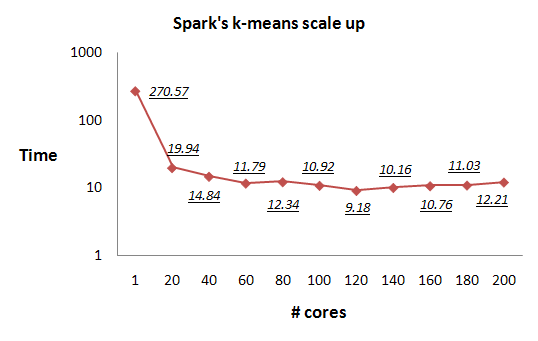
\includegraphics[width=0.5\textwidth]{kmeans-spark}
    \caption{Average time (3x) obtained for Spark's k-Means. Label values are displayed close to the points. Y-axis in 10-log scale.}
    \label{fig:kmeans-spark}
\end{figure}

Figure~\ref{fig:rf-spark} performs the same study for Random Forest. The results shows a trend similar to that in the above figure, and where the same conclusions can be stated. The global minimum can also be found in 120 cores. The only noticeable difference is the lower time cost held by Random Forest compared with the clustering technique.

\begin{figure}[htp]
    \centering
    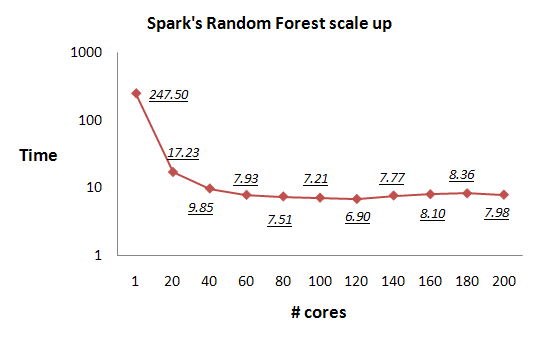
\includegraphics[width=0.5\textwidth]{rf-spark}
    \caption{Average time (3x) obtained for Spark's Random Forest. Label values are displayed close to the points. Y-axis in 10-log scale.}
    \label{fig:rf-spark}
\end{figure}

\section{Concluding Remarks}\label{sec:conclusions}

\TODO

\section*{Acknowledgments}\label{sec:ack}

This work have been partially supported by the Spanish Ministry of Science and Technology under projects TIN2014-57251-P and TIN2015-68454-R; and the Foundation BBVA project 75/2016 BigDaPTOOLS.
%\newline

%\noindent\appendix{\textbf{Bibliography}}\label{sec:biblio}

\bibliographystyle{elsarticle-num}
\bibliography{cloud,sergio}

\end{document}
